%*******************************************************************************
%****************************** Chapter Four ***********************************
%*******************************************************************************

\chapter{GP Model of TFAs}\label{ch:GP_Model_of_TFAs}

\ifpdf
    \graphicspath{{Chapter4/Figs/Raster/}{Chapter4/Figs/PDF/}{Chapter4/Figs/}}
\else
    \graphicspath{{Chapter4/Figs/Vector/}{Chapter4/Figs/}}
\fi

In this chapter we design a covariance function for reconstructing transcription factor activities given gene expression profiles and a connectivity matrix (binding data) between genes and transcription factors. Our modelling framework builds on ideas of \cite{Sanguinetti:2006} who used a linear-Gaussian state-space modelling framework to infer the transcription factor activity of a group of genes. 

We note that the TFA model with Markov property proposed by \cite{Sanguinetti:2006} is a linear Gaussian state space model which is equivalent to a Gaussian process model with a particular covariance function. We therefore build a model directly from the Gaussian process perspective to achieve the same effect. We introduce a computational trick, based on  judicious application of singular value decomposition, to enable us to efficiently fit the Gaussian process in a reduced \lq transcription factor activity\rq space. 

In the probabilistic inference of TFAs, \cite{Spellman:1998} used gene expression time series of synchronized yeast cells from the CDC-15 experiment. Two colour spotted cDNA array data set of a series of experiments to identify which genes in Yeast are cell cycle regulated. %We can make a simple helper function to plot genes from the data set (which are provided as a pandas array).

Our second data set is from ChiP-chip experiments performed on yeast by \cite{Lee:2002}. These give us the binding information between transcription factors and genes. In this thesis we are going to combine this binding information with the gene expression information to infer transcription factor activities.

\section{Model for Transcription Factor Activities}\label{sec:Model_for_TFA}
Given $\mathbf{Y} \in \mathbb{R}^{n\times T}$, is the matrix of $log$-ed gene expression, where $n$ is the number of genes, $T$ is the time points. We assume a linear (additive) model giving the relationship between the expression level of the gene and the corresponding transcription factor activity which are unobserved, but we represent by a matrix $\mathbf{F} \in \mathbb{R}^{q\times T}$, where $q$ is the number of transcription factors. Our basic assumption is as follows
\begin{enumerate}
 \item Transcription factors are in time series, so they are likely to be temporally smooth. 
 \item The transcription factors are potentially correlated with one another (to account for transcription factors that operate in unison).
\end{enumerate}

\textbf{Correlation Between Transcription Factors}: if there are $q$ transcription factors then the correlation between different transcription factors is encoded in a covariance matrix, $\boldsymbol{\Sigma}$ which is $q\times q$ in dimensionality. 

\textbf{Temporal Smoothness}: we assume that the log of the transcription factors' activities is temporally smooth, and drawn from an underlying Gaussian process with covariance $\mathbf{K}_t$. 

\textbf{Intrinsic Coregionalization Model}: we assume that the joint process across all $q$ transcription factor activities and across all time points is well represented by an intrinsic model of coregionalization where the covariance is given by the Kronecker product of these terms.
\begin{equation} \label{eq:K_intrinsic_coregionalization}
  \mathbf{K}_f = \mathbf{K}_t \otimes \boldsymbol{\Sigma}
\end{equation}

\begin{figure}[t]
	\centering
		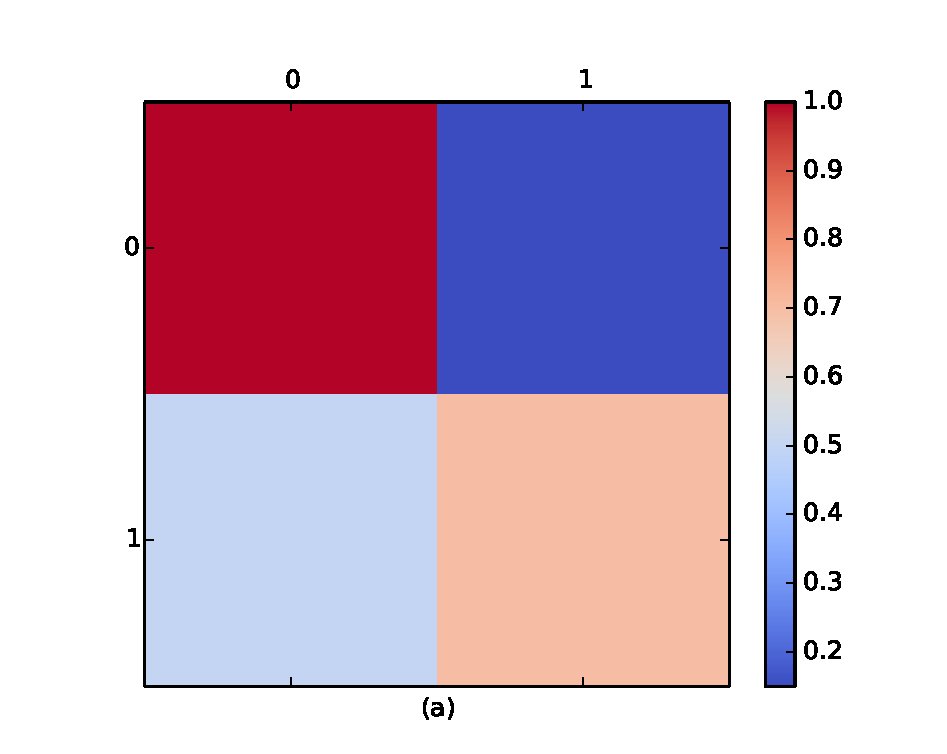
\includegraphics[width=.4\textwidth,keepaspectratio]{a.pdf}
		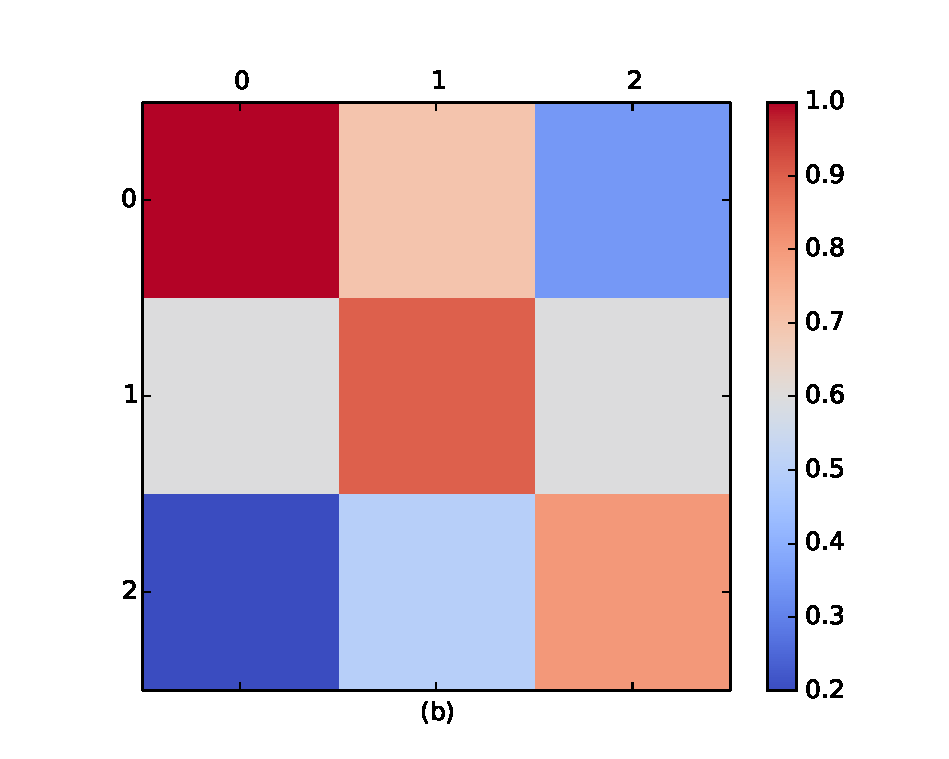
\includegraphics[width=.4\textwidth,keepaspectratio]{b.pdf}
		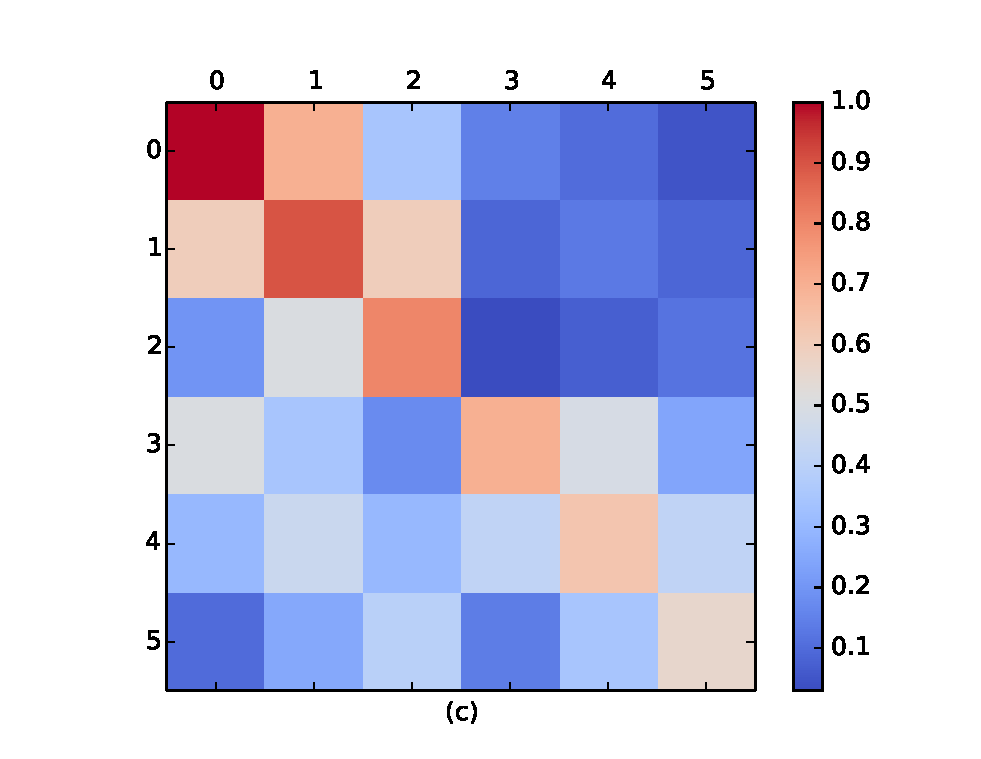
\includegraphics[width=.6\textwidth,keepaspectratio]{c.pdf}
		\rule{35em}{0.5pt}
	\caption[Demonstration of Kronecker product by tiling]{Demonstration of Kronecker product by tiling. Assume (a) represents $\textbf{K}_t$ and (b) represents $\boldsymbol{\Sigma}$ of Equation \ref{eq:K_intrinsic_coregionalization}, then the representation of $\textbf{K}_f$ will be as like (c).}
	\label{fig:kron_prod}
\end{figure}
This is known as an intrinsic coregionalization model (\cite{Wackernagel:2003}). \cite{Alvarez:2012} presented the machine learning orientated review of these methods. The matrix $\boldsymbol{\Sigma}$ is known as the coregionalization matrix. We describe the methodology of designing kernel using \emph{coregionalization} at Chapter \ref{ch:Clustering_Gene_Expression_Data} in Section \ref{subSec:Kernel_Design_with_Coregionalization}. Figure \ref{fig:kron_prod} is the realization of intrinsic model of coregionalization.

\section{Relation to Gene Expressions}
We now assume that the $j^{th}$ gene's expression is given by the product of the transcription factors that bind to that gene. Because we are working in log space, that implies a log linear relationship. At the $i^{th}$ time point, the log of the $j^{th}$ gene's expression, $\mathbf{y}_{i,j}$ is linearly related to the log of the transcription factor activities at the corresponding time point, $\mathbf{f}_{i, :}$. This relationship is given by the binding information from $\mathbf{S}$. We then assume that there is some corrupting Gaussian noise to give us the final observation.
\begin{equation} \label{eq:yij}
  \mathbf{y}_{i, j} = \mathbf{S}\mathbf{f}_{:, i} + \boldsymbol{\epsilon}_i
\end{equation}  
where the Gaussian noise is sampled from
\begin{equation} \label{eq:epsi}
  \boldsymbol{\epsilon}_i \sim \mathcal{N}(\mathbf{0}, \sigma^2 \mathbf{I})
\end{equation}

\section{Gaussian Process Model of Gene Expression}
We consider a vector operator which takes all the separate time series in $\mathbf{Y}$ and stacks the time series to form a new vector $n\times T$ length vector $\mathbf{y}$. A similar operation is applied to form a $q \times T$ length vector $\mathbf{f}$. Using Kronecker products we can now represent the relationship between $\mathbf{y}$ and $\mathbf{f}$ as follows: Standard properties of multivariate Gaussian distributions tell us that
\begin{equation} \label{eq:mGPd}
\mathbf{y} \sim \mathcal{N}(\mathbf{0}, \mathbf{K}),
\end{equation}
where
\begin{equation} \label{eq:K}
\mathbf{K} = \mathbf{K}_t \otimes \mathbf{S} \boldsymbol{\Sigma} \mathbf{S}^\top + \sigma^2 \mathbf{I}.
\end{equation}
This results in a covariance function that is of size $n$ by $T$ where $n$ is number of genes and $T$ is number of time points. However, we can get a drastic reduction in the size of the covariance function by considering the singular value decomposition (Appendix \ref{Appendix_A}, Section \ref{app_svd}) of $\mathbf{S}$. The matrix $\mathbf{S}$ is $n$ by $q$ matrix, where $q$ is the number of transcription factors. It contains a \lq 1\rq if a given transcription factor binds to a given gene, and \lq 0\rq otherwise. The likelihood of a multivariate Gaussian is
\begin{equation} \label{eq:Likelihood}
L = -\frac{1}{2} \log |\mathbf{K}| - \frac{1}{2} \mathbf{y}^\top \mathbf{K}^{-1} \mathbf{y}
\end{equation}

In the worst case, because the vector $\mathbf{y}$ contains $T\times n$ points ($T$ time points for each of $n$ genes) we are faced with $\mathcal{O}(T^3n^3)$ computational complexity. We are going to use a rotation trick to get the likelihood. 

\section{The Main Computational Trick}

\subsection{Rotating the Basis of a Multivariate Gaussian}
For any multivariate Gaussian you can rotate the data set and compute a new rotated covariance which is valid for the rotated data set. Mathematically this works by first inserting $\mathbf{R}\mathbf{R}^\top$ into the likelihood at three points as follows:
\begin{equation} \label{eq:LikelihoodRotation}
  L = -\frac{1}{2} \log |\mathbf{K}\mathbf{R}^\top\mathbf{R}| 
      - \frac{1}{2} \mathbf{y}^\top\mathbf{R}^\top\mathbf{R} \mathbf{K}^{-1}\mathbf{R}^\top\mathbf{R} \mathbf{y} 
      + \text{const}
\end{equation}
The rules of determinants and a transformation of the data allows us to rewrite the likelihood as
\begin{equation} \label{eq:LikelihoodRotationRerite}
  L = -\frac{1}{2} \log |\mathbf{R}^\top\mathbf{K}\mathbf{R}| 
      - \frac{1}{2} \hat{\mathbf{y}}^\top \left[\mathbf{R}^\top\mathbf{K}\mathbf{R}\right]^{-1}\hat{\mathbf{y}} 
      + \text{const}
\end{equation}
where we have introduced the rotated data: $\hat{\mathbf{y}}=\mathbf{R} \mathbf{y}$. 
Geometrically what this says is that if we want to maintain the same likelihood, then when we rotate our data set by $\mathbf{R}$ we need to rotate either side of the covariance matrix by $\mathbf{R}$, which makes perfect sense when we recall the properties of the multivariate Gaussian. 

\subsection{A Kronecker Rotation}
In this thesis we are using a particular structure of covariance which involves a Kronecker product. The rotation we consider will be a Kronecker rotation (\cite{Stegle:2011}). We are going to try and take advantage of the fact that the matrix $\mathbf{S}$ is square meaning that $\mathbf{S}\boldsymbol{\Sigma}\mathbf{S}^\top$ is not full rank (it has rank of most $q$, but is size $n\times n$, and we expect number of transcription factors $q$ to be less than number of genes $n$). 

When ranks are involved, it is always a good idea to look at singular value decompositions (SVDs). The SVD of $\mathbf{S}$ is given by:
\begin{equation} \label{eq:SVD}
\mathbf{S} = \mathbf{Q} \boldsymbol{\Lambda} \mathbf{V}^\top
\end{equation}
where $\mathbf{V}^\top \mathbf{V} = \mathbf{I}$, $\boldsymbol{\Lambda}$ is a diagonal matrix of positive values, $\mathbf{Q}$ is a matrix of size $n\times q$: it matches the dimensionality of $\mathbf{S}$, and we have $\mathbf{Q}^\top \mathbf{Q} = \mathbf{I}$. Note that because it is not square, $\mathbf{Q}$ is not in itself a rotation matrix. However it could be seen as the first $q$ columns of an $n$ dimensional rotation matrix (assuming $n$ is larger than $q$, i.e. there are more genes than transcription factors). 

If we call the $n-q$ missing columns of this rotation matrix $\mathbf{U}$ then we have a valid rotation matrix $\mathbf{R}=\begin{bmatrix} \mathbf{Q}& \mathbf{U}\end{bmatrix}$. Although this rotation matrix is only rotating across the $n$ dimensions of the genes, not the additional dimensions across time. In other words we are choosing $\mathbf{K}_t$ to be unrotated. To represent this properly for our covariance we need to set $\mathbf{R} = \mathbf{I} \otimes \begin{bmatrix} \mathbf{Q}& \mathbf{U}\end{bmatrix}$. This gives us a structure that when applied to a covariance of the form $\mathbf{K}_t\otimes \mathbf{K}_n$ it will rotate $\mathbf{K}_n$ whilst leaving $\mathbf{K}_t$ untouched.

When we apply this rotation matrix to $\mathbf{K}$ we have to consider two terms, the rotation of $\mathbf{K}_t \otimes \mathbf{S}\boldsymbol{\Sigma}\mathbf{S}^\top$, and the rotation of $\sigma^2 \mathbf{I}$.

Rotating the latter is easy, because it is just the identity matrix multiplied by a scalar so it remains unchanged 
\begin{equation} \label{eq:RotatingNoise}
\mathbf{R}^\top\mathbf{I}\sigma^2 \mathbf{R}= \mathbf{I}\sigma^2
\end{equation}
The former is slightly more involved, for that term we have
\begin{equation} \label{eq:svdONK}
\left[\mathbf{I}\otimes \begin{bmatrix}\mathbf{Q} & \mathbf{U}\end{bmatrix}^\top \right]\mathbf{K}_t \otimes 
\mathbf{S}\boldsymbol{\Sigma}\mathbf{S}^\top
\left[ \mathbf{I} \otimes \begin{bmatrix}\mathbf{Q} & \mathbf{U}\end{bmatrix}\right]
=
\mathbf{K}_t \otimes \begin{bmatrix}\mathbf{Q} & \mathbf{U}\end{bmatrix}^\top 
\mathbf{S} \boldsymbol{\Sigma}\mathbf{S}^\top \begin{bmatrix}\mathbf{Q} & \mathbf{U}\end{bmatrix}.
\end{equation}
Since $\mathbf{S} = \mathbf{Q}\boldsymbol{\Lambda}\mathbf{V}^\top$ then we have
\begin{equation} \label{eq:yqprime}
  \begin{bmatrix}\mathbf{Q} & \mathbf{U}\end{bmatrix}^\top \mathbf{S}\boldsymbol{\Sigma}\mathbf{S}^\top\begin{bmatrix}\mathbf{Q} & \mathbf{U}\end{bmatrix} 
    = 
  \begin{bmatrix}\boldsymbol{\Lambda} \mathbf{V}^\top \boldsymbol{\Sigma}\mathbf{V} \boldsymbol{\Lambda} &\mathbf{0} \\ \mathbf{0} & \mathbf{0}\end{bmatrix}.
\end{equation}
This prompts us to split our vector $\hat{\mathbf{y}}$ into a $q$ dimensional vector $\hat{\mathbf{y}}_u = \mathbf{U}^\top \mathbf{y}$ and an $n-q$ dimensional vector $\hat{\mathbf{y}}_q =\mathbf{Q}^\top \mathbf{y}$. The Gaussian likelihood can be written as
\begin{equation} \label{eq:LikelihoodParts}
L = L_u + L_q + \text{const}
\end{equation}
where
\begin{equation} \label{eq:Lq}
L_q = -\frac{1}{2} \log |\mathbf{K}_t\otimes
	  \boldsymbol{\Lambda}\mathbf{V}^\top\boldsymbol{\Sigma}\mathbf{V}\boldsymbol{\Lambda}+\sigma^2\mathbf{I}| 
	- \frac{1}{2} \hat{\mathbf{y}}_q^\top \left[\mathbf{K}_t\otimes 
	  \boldsymbol{\Lambda}\mathbf{V}^\top\boldsymbol{\Sigma}\mathbf{V}\boldsymbol{\Lambda}+\sigma^2\mathbf{I}\right]^{-1} \hat{\mathbf{y}}_q
\end{equation}
and
\begin{equation} \label{eq:Lu}
L_u = -\frac{T(n-q)}{2} \log \sigma^2  -\frac{1}{2\sigma^2} \hat{\mathbf{y}}_u^\top \hat{\mathbf{y}}_u
\end{equation}

Strictly speaking we should fit these models jointly, but for the purposes of illustration we will firstly use a simple procedure. Firstly, we fit the noise variance $\sigma^2$ on $\hat{\mathbf{y}}_u$ alone using $L_u$. Once this is done, fix the value of $\sigma^2$ in $L_q$ and optimize with respect to the other parameters.

With the current design the model is switching off the temporal correlation. The next step in the analysis will be to reimplement the same model as described by \cite{Sanguinetti:2006} and recover their results. That will involve using an Ornstein-Uhlenbeck covariance (we proved the rationale behind the choice of the covariance function in Chapter \ref{ch:GaussianProcessRegression} Sec \ref{Sec:Toward_TFA}) and joint maximisation of the likelihood of $L_u$ and $L_q$.

\section{Making Prediction}
\begin{figure}[t]
	\centering
		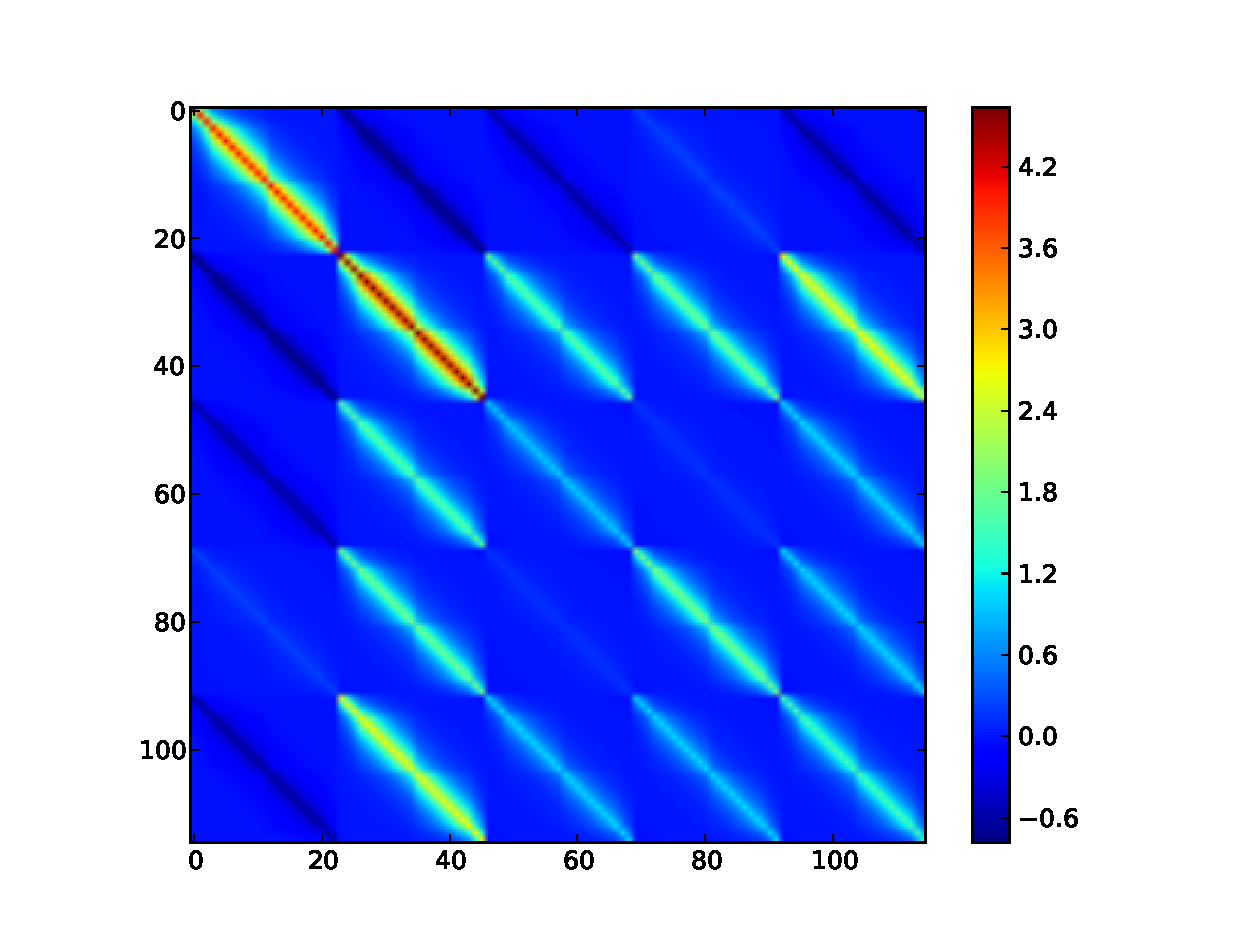
\includegraphics[width=\textwidth,keepaspectratio]{kern_6TF.eps}
		\rule{35em}{0.5pt}
	\caption[Kernel of intrinsic coregionalization model $\textbf{K}_f$ considering 5 transcription factors where covariance matrix $\boldsymbol{\Sigma}$ was constructed using Ornstein-Uhlenbeck kernel and White kernel in additive form] {Kernel of Intrinsic Coregionalization model $\textbf{K}_f$ considering 5 transcription factors where covariance matrix $\boldsymbol{\Sigma}$ of $\left( Equation \ref{eq:K} \right)$ was constructed using Ornstein-Uhlenbeck kernel and White kernel in additive form.}
	\label{fig:kern_6TF}
\end{figure}
Using Kronecker product we can rewrite the Equation \ref{eq:mGPd} as:
\begin{equation} \label{eq:predicYq}
  \mathbf{y_q}  \sim \mathcal{N} \left( \mathbf{0}, 
    \mathbf{K}_{t,t} \otimes \boldsymbol{\Lambda} \mathbf{V}^T\boldsymbol{\Sigma} \mathbf{V} \boldsymbol{\Lambda} +
    \sigma^2\mathbf{I}\right)
\end{equation}
Standard properties of multivariate Gaussian distributions tells us can split equation \ref{eq:predicYq} into
\begin{equation} \label{eq:gEp}
  \mathbf{y_q} = \mathbf{g} + \boldsymbol{\epsilon}
\end{equation}
where $\mathbf{g}$ and $\boldsymbol{\epsilon}$ are also Gaussian distributions and can be represented by:
\begin{equation}\label{eq:g}
  \mathbf{g} \sim \mathcal{N} \left( \mathbf{0}, 
    \mathbf{K}_{t,t} \otimes 
    \boldsymbol{\Lambda} \mathbf{V}^T\boldsymbol{\Sigma} \mathbf{V} \boldsymbol{\Lambda} \right)
\end{equation}
\begin{equation}\label{eq:Epsi}
  \boldsymbol{\epsilon} \sim \mathcal{N} \left(\mathbf{0},\sigma^2\mathbf{I}\right)
\end{equation}
Now we can represent the matrix $\mathbf{F}$ of transcription factor activity as:
\begin{equation}\label{eq:F}
  \mathbf{F} = \mathbf{I} \otimes \mathbf{V} \Lambda^{-1} \mathbf{g}
\end{equation}
\begin{equation}\label{eq:Sigma}
  \boldsymbol{\Sigma} = \mathbf{W}\mathbf{W}^T + \text{diag}\left(\boldsymbol{\kappa}\right)
\end{equation}
where $\boldsymbol{\kappa}$ is the kappa value from coregionalization matrix.
\begin{equation} \label{eq:predictionF}
  \mathbf{F}  \sim \mathcal{N} \left( \mathbf{0},\mathbf{K}_{t,t} \otimes \boldsymbol{\Sigma}\right)
\end{equation}
Now we can find the conditional distribution of $\mathbf{g}$ for given $\mathbf{y}_q$ by
\begin{equation}\label{eq:gGivenYq}
 p\left(\mathbf{g} \middle| \mathbf{y}_q\right) \sim 
    \mathcal{N} \left( \boldsymbol{\mu}_g, \mathbf{C}_g\right)
\end{equation}
with a mean given by
\begin{equation} \label{eq:prediction_MuG}
  \boldsymbol{\mu}_g = 
    \left[ \mathbf{K}_{t_\star,t} \otimes \boldsymbol{\Lambda} \mathbf{V}^T\boldsymbol{\Sigma} \mathbf{V} \boldsymbol{\Lambda}  \right] 
    \left[ \mathbf{K}_{t,t} \otimes \boldsymbol{\Lambda} \mathbf{V}^T\boldsymbol{\Sigma} \mathbf{V} \boldsymbol{\Lambda} + \sigma^2 \mathbf{I} \right]^{-1}\mathbf{y}_q
\end{equation}
and the covariance given by
\begin{equation} \label{eq:prediction_Cg}
\begin{split}
\boldsymbol{C}_g &= 
    \left[ \mathbf{K}_{t_\star,t_\star} \otimes \boldsymbol{\Lambda} \mathbf{V}^T\boldsymbol{\Sigma} \mathbf{V} \boldsymbol{\Lambda}  \right] \\
    & -\left[ \mathbf{K}_{t_\star,t} \otimes \boldsymbol{\Lambda} \mathbf{V}^T\boldsymbol{\Sigma} \mathbf{V} \boldsymbol{\Lambda}  
    \left[ \mathbf{K}_{t,t} \otimes \boldsymbol{\Lambda} \mathbf{V}^T\boldsymbol{\Sigma} \mathbf{V} \boldsymbol{\Lambda} + \sigma^2 \mathbf{I} \right]^{-1} 
    \mathbf{K}_{t_\star,t} \otimes \boldsymbol{\Lambda} \mathbf{V}^T\boldsymbol{\Sigma} \mathbf{V} \boldsymbol{\Lambda} \right]
\end{split}
\end{equation}
\begin{figure}[t]
	\centering
		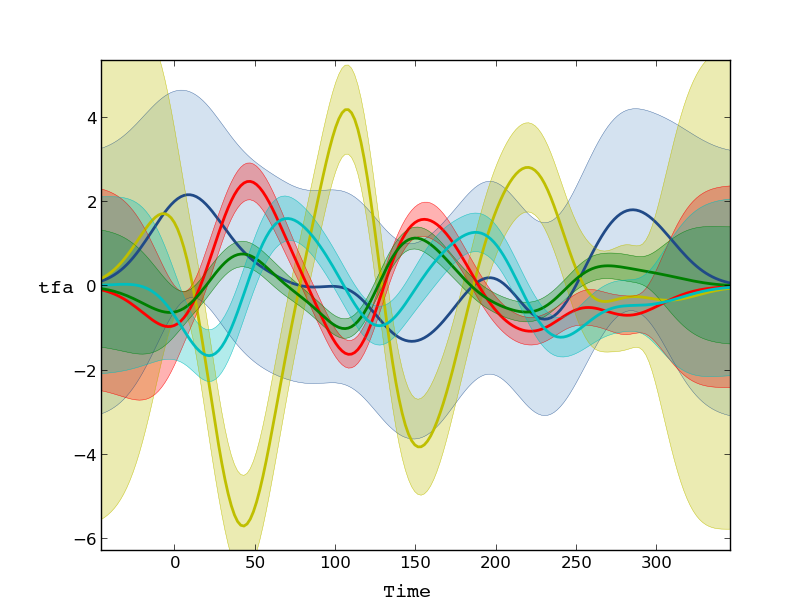
\includegraphics[width=0.9\textwidth,keepaspectratio]{RBFWh9TF.png}
		\rule{35em}{0.5pt}
	\caption[Variation of activities of transcription factors with exponentiated quadratic kernel and  white kernel in additive form] {Variation of activities of Transcription factors with exponentiated quadratic kernel and  white kernel in additive form. Solid line represents a posterior mean and shaded area represents the 95\% confidence interval. Different color show the transcription factor activity of randomly picked transcription factors.}
	\label{fig:TFA_with_RBFnWhKernel}
\end{figure}
Finally the posterior mean of the conditional distribution  is %of Equation \ref{eq:predicYq} %\ref{eq:predictionTFA} 
is
\begin{equation} \label{eq:prediction_MuF}
  \boldsymbol{\mu}_F = 
    \mathbf{K}_{t_\star,t} \otimes \boldsymbol{\Sigma} \mathbf{V} \boldsymbol{\Lambda}
    \left[ \mathbf{K}_{t,t} \otimes \boldsymbol{\Lambda} \mathbf{V}^T\boldsymbol{\Sigma} \mathbf{V} \boldsymbol{\Lambda} + \sigma^2 \mathbf{I} \right]^{-1}\mathbf{y}_q
\end{equation}
and the covariance of the conditional distribution is %of Equation \ref{eq:predicYq} given by
\begin{equation} \label{eq:prediction_CF}
\begin{split}
  \boldsymbol{C}_F &= 
    \mathbf{K}_{t_\star,t_\star} \otimes \boldsymbol{\Sigma} \\
    & - \mathbf{K}_{t_\star,t} \otimes \boldsymbol{\Sigma}\mathbf{V} \boldsymbol{\Lambda}
    \left[ \mathbf{K}_{t,t} \otimes \boldsymbol{\Lambda} \mathbf{V}^T\boldsymbol{\Sigma} \mathbf{V} \boldsymbol{\Lambda} + \sigma^2 \mathbf{I} \right]^{-1} 
    \left[ \mathbf{K}_{t_\star,t} \otimes \boldsymbol{\Lambda} \mathbf{V}^T\boldsymbol{\Sigma}\right]
\end{split}
\end{equation}
Figure \ref{fig:kern_6TF} shows the pictorial representation of intrinsic coregionalization kernel (Equation \ref{eq:K}) $\textbf{K}_f$ considering 20 transcription factors where covariance matrix $\boldsymbol{\Sigma}$ of  was constructed using Ornstein-Uhlenbeck kernel and white kernel in additive form.


\section{Dataset and Result analysis}
\begin{figure}[t]
	\centering
		%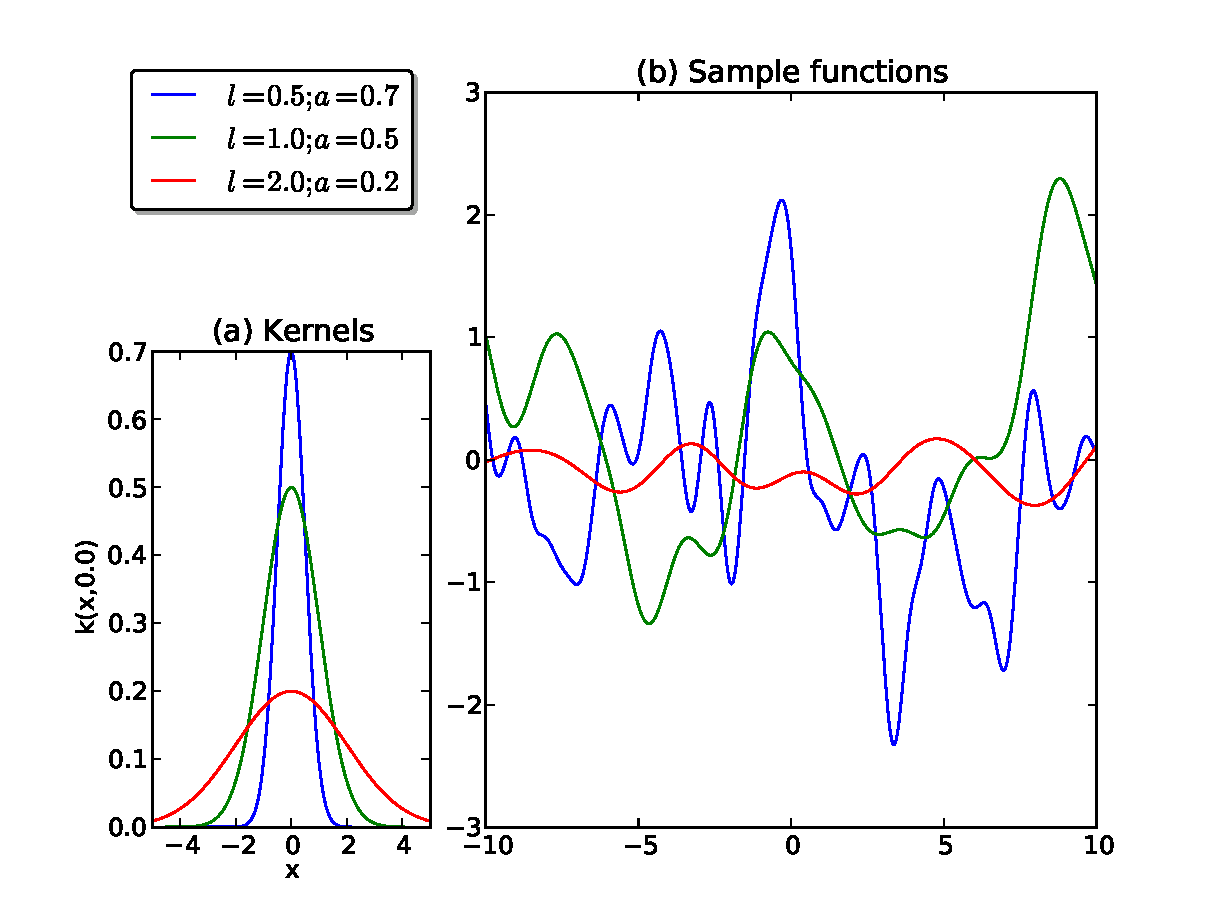
\includegraphics[width=10cm,keepaspectratio]{diagrams/SE_cov.pdf}
		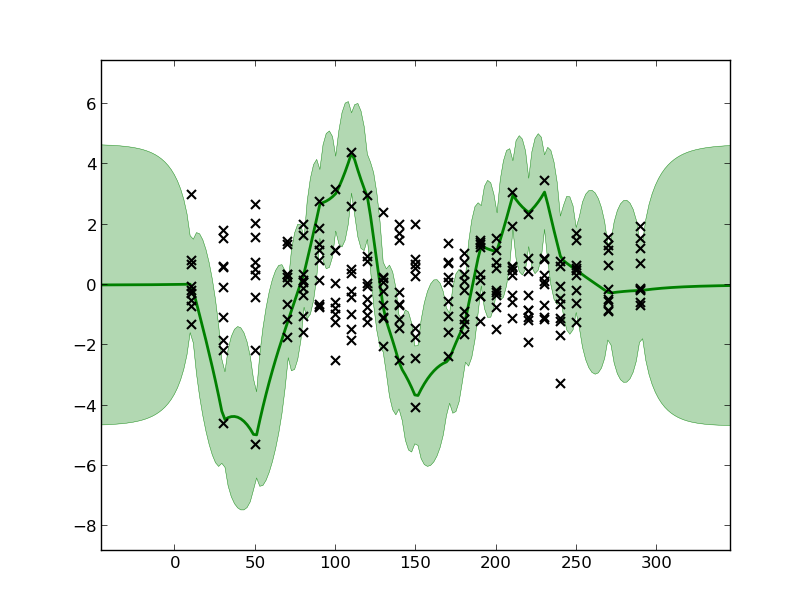
\includegraphics[width=0.9\textwidth,keepaspectratio]{ACE2_OU_Wh_9TF.png}
		\rule{35em}{0.5pt}
	\caption[Transcription factor activity of ACE2]
		{Transcription factor activity of ACE2. Solid line represents a posterior mean and shaded area represents 95\% confidence interval. $x$-axis represents the time and $y$-axis represent the transcription factor activity.}
	\label{fig:TFA_of_of_ACE2}
\end{figure}
\begin{figure}
	\centering
		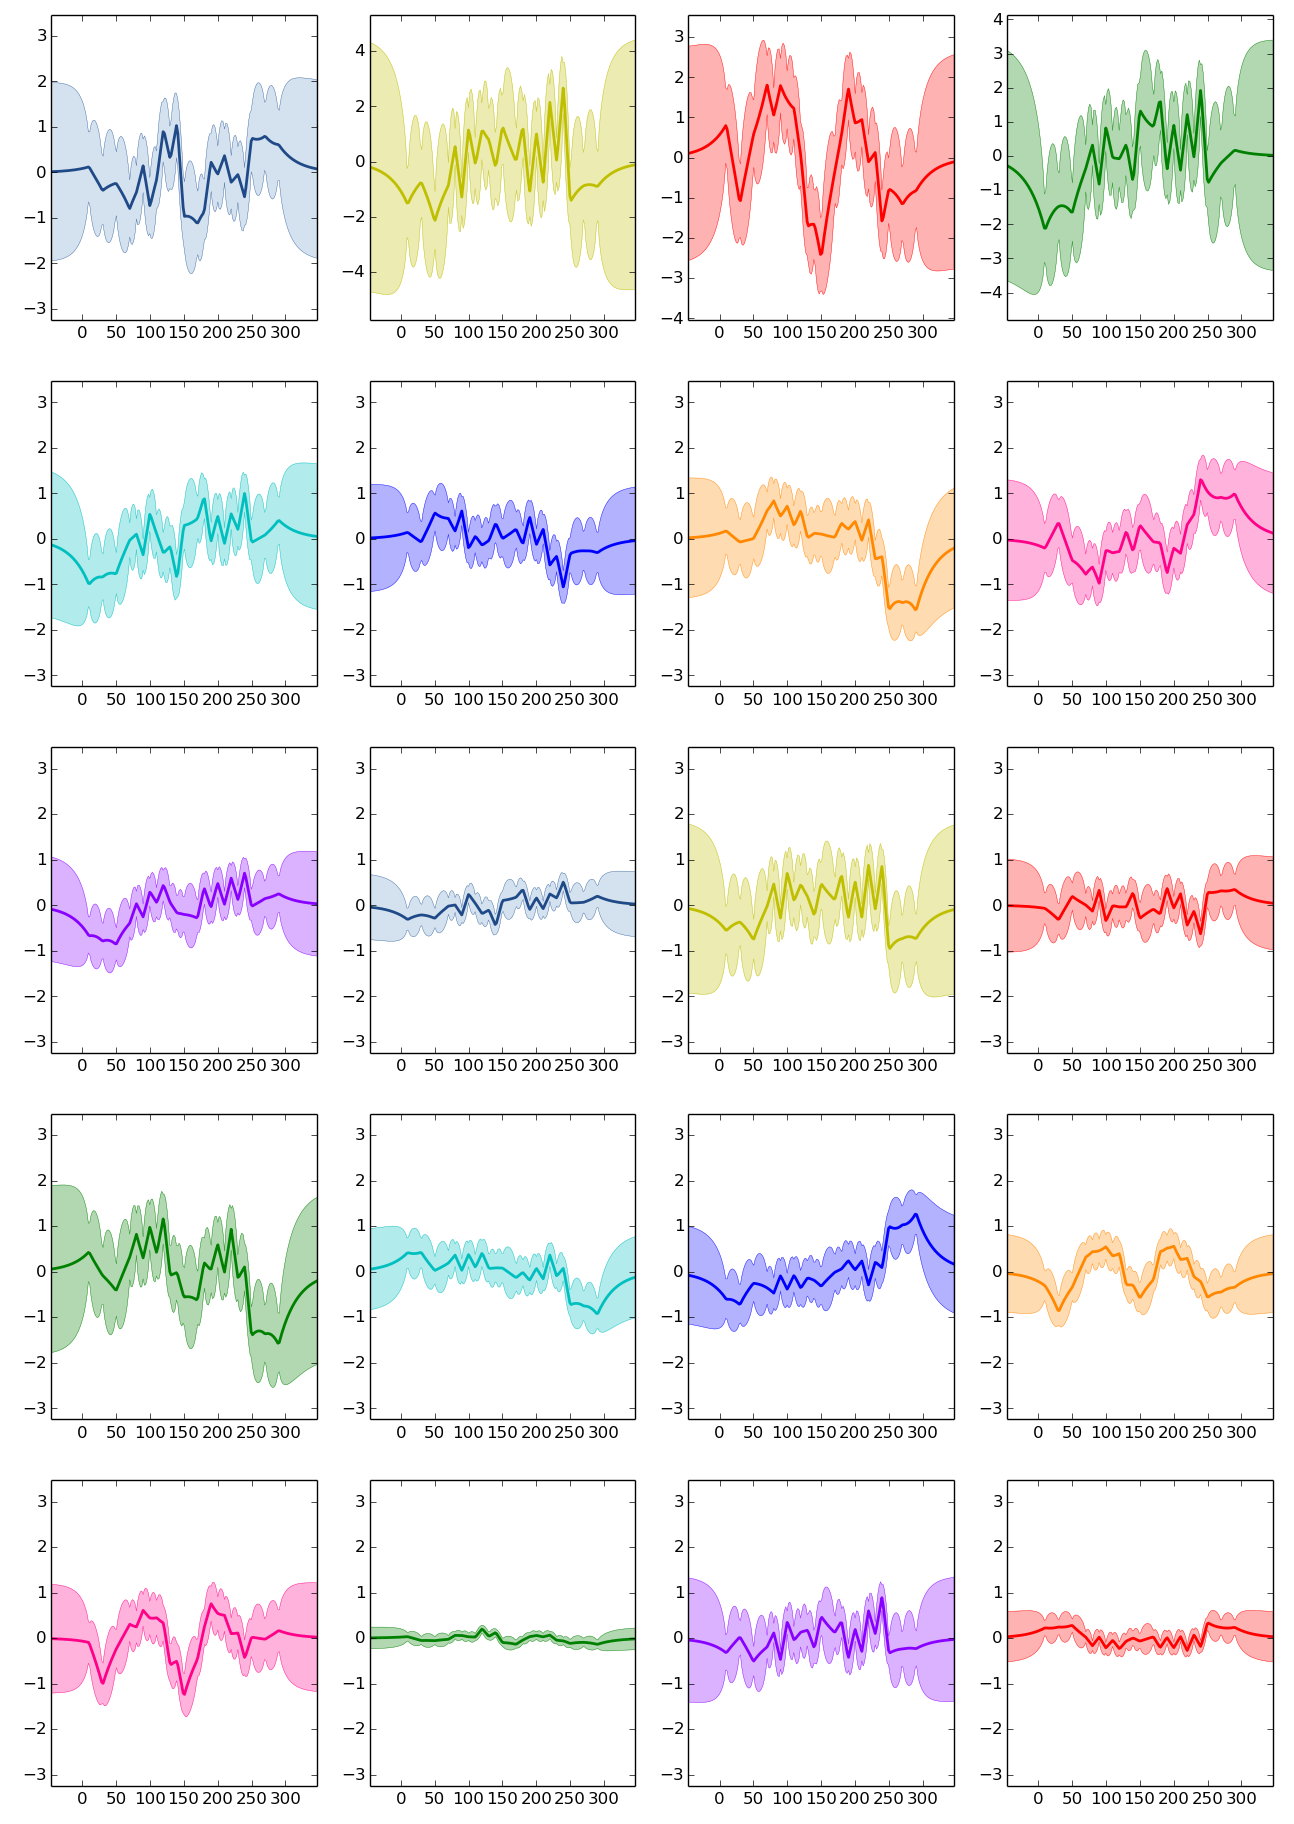
\includegraphics[width=.95\textwidth,keepaspectratio]{OU20TF2.png}
		\rule{35em}{0.5pt}
	\caption[Transcription factor activity of different transcription factor]{Transcription factor activity of different transcription factors: individual plots shows the activity of the transcription factor. Here, solid line represents a posterior mean and shaded area represents the 95\% confidence interval. $x$-axis represents the time and $y$-axis represent the TFA.}
	\label{fig:TFA_of_20TF}
\end{figure}

Here in this experiment we used the classic \cite{Spellman:1998} yeast cell cycle dataset. The \emph{cdc15} time series data has 23 time points. 

Exponentiated quadratic kernel is very smooth kernel compared to Ornstein-Uhlenbeck kernel and perhaps is not a very good choice for the determination of actual transcription factors activities. Still it can figure out the basic nature of the activities with over smoothness. Figure \ref{fig:TFA_with_RBFnWhKernel} shows activities of different transcription factors while the model was developed considering exponentiated quadratic kernel with White kernel in additive form.

Figure \ref{fig:TFA_of_of_ACE2} shows transcription factor activity of ACE2. While developing the model we chose Ornstein-Uhlenbeck kernel and White kernel in additive form. We believe that the Ornstein-Uhlenbeck kernel will consider the basic nature of the transcription factors activity while White kernel will deal the noise associated the collected gene expression data.

Figure \ref{fig:TFA_of_20TF} transcription factor activity of different (arbitrarily chosen) transcription factors  where we used our newly developed model. Here, as a prior we used Ornstein-Uhlenbeck kernel and White kernel. In the plot, a solid line represents a posterior mean and shaded area represents the 95\% confidence interval.

%TODO
\section{Discussion}
At Chapter \ref{ch:GaussianProcessRegression} Section \ref{Sec:Toward_TFA} we noted that the linear Gaussian model is equivalent to a Gaussian process with a particular covariance function. In this chapter we therefore build a model directly from the Gaussian process perspective. Here we designed a covariance function for reconstructing transcription factor activities given gene expression profiles and a connectivity information between genes and transcription factors. In the beginning section (Sec \ref{sec:Model_for_TFA}) of the chapter we assumed that the joint process across all transcription factor activities and across all time points might have some correlation, hence we introduced intrinsic model of coregionalization for the the joint process. We also introduced a computational trick, based on  judicious application of singular value decomposition, to enable us to efficiently fit the Gaussian process in a reduced \lq TF activity\rq  space. 
